We have designed P2P-Tube as a video sharing platform based on NextShare video streaming capabilities. Currently there are two browser plugins for video rendering developed by P2P-Next to be NextShare compliant. The first of them, known as SwarmPlayer, is based on HTML5 video tag. Because HTML5 is still a draft and older browsers do not support it, another NextShare plugin based on VLC has been created, named NextSharePC. P2P-Tube supports both versions of NextShare plugins and users can choose which to use directly from the watching page.

Within the platform video assets can be grouped in categories, facilitating easier browsing. Searching by keywords is also possible, both in the whole set of videos or in a specific category. Search results are ordered by relevance. Users can sign up for an account and singing in is possible with internal P2P-Tube authentication, with LDAP or with OpenID. Logged in users can comment video assets and once a day for each video can rate it with a Like or a Dislike.

Users can upload video assets through an upload mechanism described in the next subsection.

\subsection{Content Ingestion}
\label{subsec:content-ingestion}

NextSharePC can play any video format as long as VLC supports it. SwarmPlayer supports only video containers and codecs which are compliant with HTML5. Most modern browsers support videos having Ogg containers with Vorbis audio codec and Theora video codec or WebM containers with Vorbis audio codec and VP8 video codec. Users must be able to upload videos in a format of their choice like MPEG, DivX or AVC/H.264. Thus, the platform must perform a conversion from the input user format to a NextShare compliant format. P2P-Tube converts all videos to Ogg with Vorbis and Theora in order to be compatible with most modern browsers and to make video assets playable with any of the two NextShare plugins. However this can be changed from the platform configuration.

Besides video conversion, several other operations must be performed in order to make the new video available on the platform. All this is done by a \textbf{Content Ingestion Server} (\textbf{CIS}) which is typically located on a different machine.

\begin{figure}[h]
  \begin{center}
    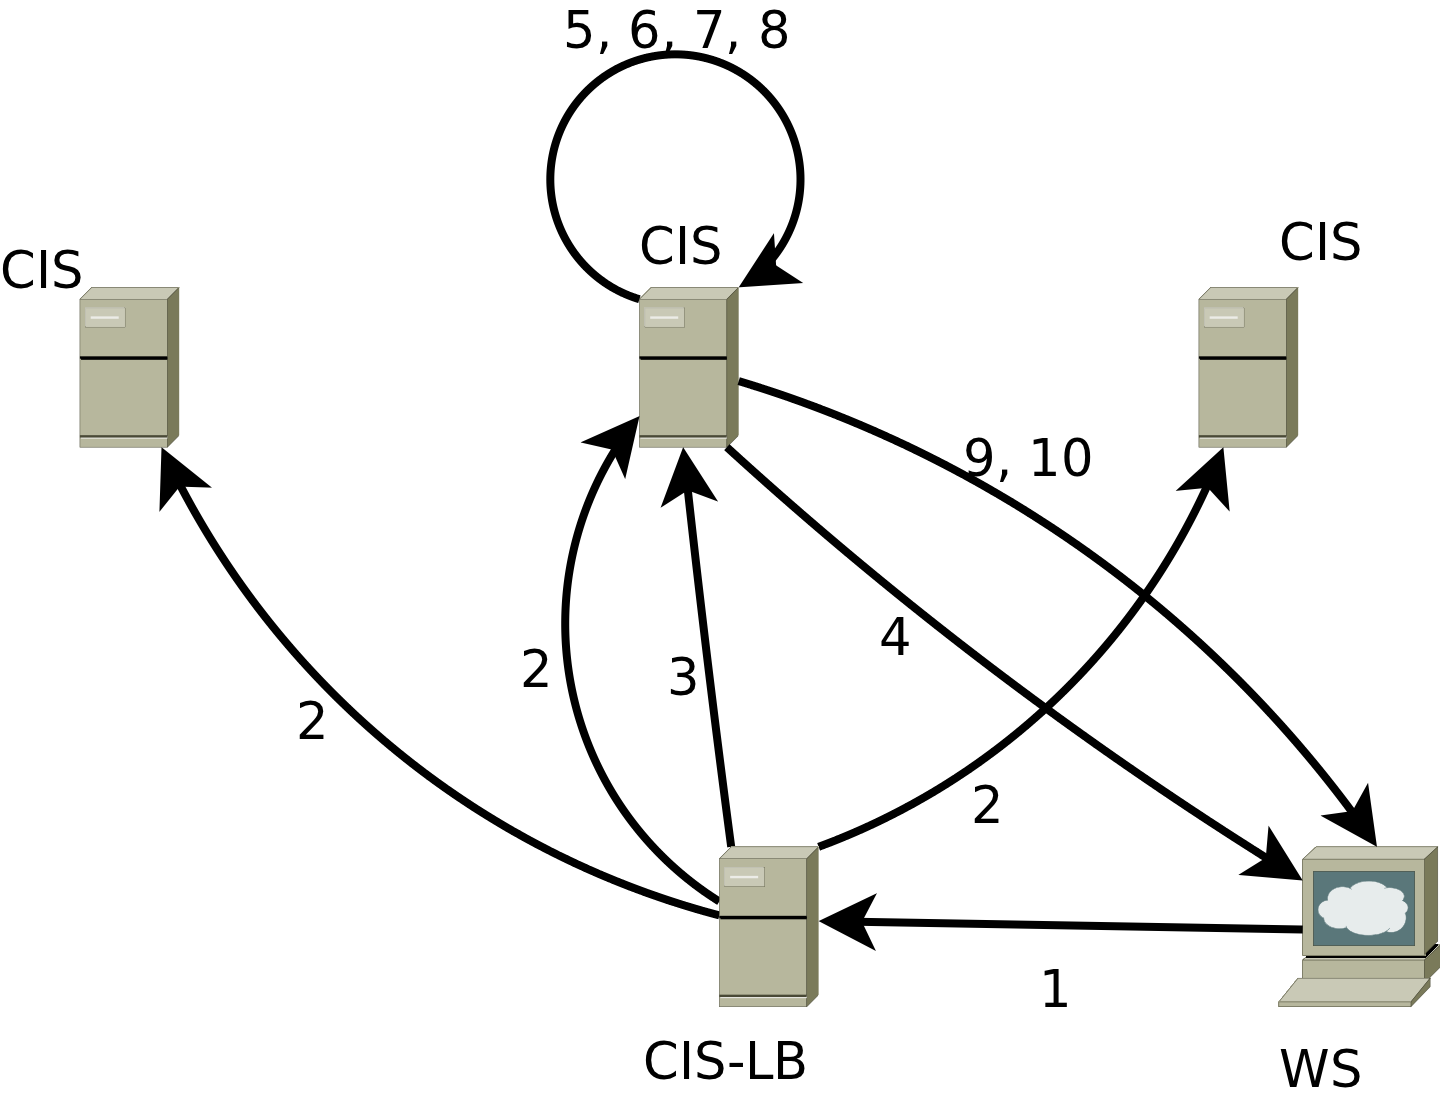
\includegraphics[width=\columnwidth]{img/content-ingestion.png}
  \end{center}
  \caption{Content Ingestion Process}
  \label{fig:content-ingestion}
\end{figure}

An user uploads a video file (referred here as \textit{raw video file}) to a the web server and may also provide additional information about it, like title, description, tags etc.. When the video upload finishes the process of content ingestion is started by the Web Server by sending a content ingestion request to a CIS. This can be done directly if in the system is a single CIS or indirectly via a CIS Load Balancer (CIS-LB), which forwards the request to one CIS from a pool of CIS machines. By doing load balancing, the indirect request method provides more scalability by offering the opportunity of running more content ingestion jobs in parallel, allowing more users to add content simultaneously. This also increases availability by making the system fault tolerant in case of CIS faults.

CIS operation through a CIS Load Balancer is described in Figure \ref{fig:content-ingestion}. Until the end of this subsection, the numbers in brackets refer to the arrows from the figure. The web server sends a \textbf{content ingestion request} to CIS-LB (1), which must choose the least loaded CIS from the system. To do this it queries each CIS for its load by sending a \textbf{get load request} (2) and establishes by processing the answer which one is the least loaded. The content ingestion request previously received is then forwarded to the least loaded CIS (3), informing it about the new video file that has been uploaded. The message also contains information about one or more formats in which the video must be converted referred here as \textit{destination formats}. This information includes parameters for each format like image resolution, frame rate, audio quality etc.. The least loaded CIS which received the request executes a job on the raw video file uploaded by doing the following operations:

\begin{itemize}
 \item \textbf{Transfers locally} (4) the raw video file from the web server.
 \item \textbf{Transcodes} (5) the raw video file to one or more \textit{destination formats} resulting \textit{transcoded video files}.
 \item \textbf{Extracts image thumbnails} (6) from the raw video file.
 \item \textbf{Creates torrent files} (7) (\textit{.tstream}) for transcoded video files.
 \item \textbf{Seeds} (8) the transcoded video files by using the torrent files previously created.
 \item \textbf{Transfers back} (9) torrent files and image thumbnails to the web server.
 \item Notifies the Web Server of the \textbf{job completion} (10) so that it can make the video accessible to the users.
\end{itemize}

In the end of the content ingestion process all other Content Ingestion Servers from the system must be aware of the new torrent files in order to seed them. This can be achieved by putting all torrent file in a distributed files system.